%% This is file `elsarticle-template-2-harv.tex',
%%
%% Copyright 2009 Elsevier Ltd
%%
%% This file is part of the 'Elsarticle Bundle'.
%% ---------------------------------------------
%%
%% It may be distributed under the conditions of the LaTeX Project Public
%% License, either version 1.2 of this license or (at your option) any
%% later version.  The latest version of this license is in
%%    http://www.latex-project.org/lppl.txt
%% and version 1.2 or later is part of all distributions of LaTeX
%% version 1999/12/01 or later.
%%
%% The list of all files belonging to the 'Elsarticle Bundle' is
%% given in the file `manifest.txt'.
%%
%% Template article for Elsevier's document class `elsarticle'
%% with harvard style bibliographic references
%%
%% $Id: homonym.tex,v 1.18 2010/04/28 03:08:16 jtduda Exp $
%% $URL: http://lenova.river-valley.com/svn/elsbst/trunk/elsarticle-template-2-harv.tex $
%%
%\documentclass[review,authoryear,preprint,12pt]{elsarticle}
\documentclass[final,authoryear,5p,times,twocolumn]{elsarticle}

%% Use the option review to obtain double line spacing
%% \documentclass[authoryear,preprint,review,12pt]{elsarticle}

%% Use the options 1p,twocolumn; 3p; 3p,twocolumn; 5p; or 5p,twocolumn
%% for a journal layout:
%% \documentclass[final,authoryear,1p,times]{elsarticle}
%%\documentclass[final,authoryear,1p,times,twocolumn]{elsarticle}
%% \documentclass[final,authoryear,3p,times]{elsarticle}
%%\documentclass[final,authoryear,3p,times,twocolumn]{elsarticle}
%% \documentclass[final,authoryear,5p,times]{elsarticle}
%%\documentclass[final,authoryear,5p,times,twocolumn]{elsarticle}

%% if you use PostScript figures in your article
%% use the graphics package for simple commands
%% \usepackage{graphics}
%% or use the graphicx package for more complicated commands
%% \usepackage{graphicx}
%% or use the epsfig package if you prefer to use the old commands
%% \usepackage{epsfig}

%% The amssymb package provides various useful mathematical symbols
\usepackage{amssymb}
%% The amsthm package provides extended theorem environments
%% \usepackage{amsthm}

%% The lineno packages adds line numbers. Start line numbering with
%% \begin{linenumbers}, end it with \end{linenumbers}. Or switch it on
%% for the whole article with \linenumbers after \end{frontmatter}.
%% \usepackage{lineno}

%% natbib.sty is loaded by default. However, natbib options can be
%% provided with \biboptions{...} command. Following options are
%% valid:

%%   round  -  round parentheses are used (default)
%%   square -  square brackets are used   [option]
%%   curly  -  curly braces are used      {option}
%%   angle  -  angle brackets are used    <option>
%%   semicolon  -  multiple citations separated by semi-colon (default)
%%   colon  - same as semicolon, an earlier confusion
%%   comma  -  separated by comma
%%   authoryear - selects author-year citations (default)
%%   numbers-  selects numerical citations
%%d    super  -  numerical citations as superscripts
%%   sort   -  sorts multiple citations according to order in ref. list
%%   sort&compress   -  like sort, but also compresses numerical citations
%%   compress - compresses without sorting
%%   longnamesfirst  -  makes first citation full author list
%%
%% \biboptions{longnamesfirst,comma}

% \biboptions{}

\journal{NeuroImage}

\begin{document}

\begin{frontmatter}

%% Title, authors and addresses

%% use the tnoteref command within \title for footnotes;
%% use the tnotetext command for the associated footnote;
%% use the fnref command within \author or \address for footnotes;
%% use the fntext command for the associated footnote;
%% use the corref command within \author for corresponding author footnotes;
%% use the cortext command for the associated footnote;
%% use the ead command for the email address,
%% and the form \ead[url] for the home page:
%%
%% \title{Title\tnoteref{label1}}
%% \tnotetext[label1]{}
%% \author{Name\corref{cor1}\fnref{label2}}
%% \ead{email address}
%% \ead[url]{home page}
%% \fntext[label2]{}
%% \cortext[cor1]{}
%% \address{Address\fnref{label3}}
%% \fntext[label3]{}

\title{Structural and functional connectivity influence decision-making in communication.}

%% use optional labels to link authors explicitly to addresses:
%% \author[label1,label2]{<author name>}
%% \address[label1]{<address>}
%% \address[label2]{<address>}

\author[BE]{Jeffrey T. Duda\corref{cor1}}
\cortext[cor1]{Corresponding author}
\ead{jtduda@seas.upenn.edu}
\author[Neu]{Corey T. McMillan}
\author[Neu]{Murray Grossman}
\author[Rad]{James C. Gee}
\address[BE]{University of Pennsylvania, Department of Bioengineering, Philadelphia, PA}
\address[Neu]{University of Pennsylvania Medical Center, Department of Neurology, Philadelphia, PA}
\address[Rad]{University of Pennsylvania Medical Center, Department of Radiology, Philadelphia, PA}

\begin{abstract}
The brain's language network has been the focus of much research relating function to underlying structure, although assessments of white matter connectivity within the language network have been rare. In this study, we examine measures from event-related functional MRI (fMRI) and integrate these with diffusion tensor imaging tractography and cognitive performance in healthy, right-handed control subjects. A decision-making task concerned with lexical selection involving homonyms was used to recruit a large-scale language network via fMRI. Diffusion tensor tractography was used to identify the fiber tracts that project between the nodes of the activated network, and the average fractional anisotropy was measured in each of these fiber tracts. Functional connectivity between regions was measured by correlating region-averaged fMRI event signals between pairs of regions connected by these fiber tracts. Stepwise multiple linear regression analysis was then used to identify the functional and structural connections that most significantly account for homonym selection performance. Analyses of both structural and functional networks suggest that performance depends on the integration of language and decision-making subnetworks during task performance. Moreover, we observed good convergence across these two types of analyses of network connectivity.  This work begins to provide a mechanistic account for connectivity within a large-scale neural network underlying complex human cognitive activity.

\end{abstract}

\begin{keyword}
Diffusion-weighted imaging \sep Tractography \sep Language \sep Connectivity \sep Network

%% keywords here, in the form: keyword \sep keyword

%% MSC codes here, in the form: \MSC code \sep code
%% or \MSC[2008] code \sep code (2000 is the default)

\end{keyword}

\end{frontmatter}

%\linenumbers

%% main text
\section{Introduction}
\label{Intro}


\section{Methods}
\subsection{Participants}
18 healthy young adults (11 female; mean age=25.3 years; mean education=15.1 years) from the University of Pennsylvania community participated in the study for monetary payment.  All participants were native speakers of English, right-handed, and in good health with no history of neurological or psychiatric difficulty.  Informed consent was obtained from all participants according to a protocol approved by the University of Pennsylvania Institutional Review Board.  We excluded two participants from our analyses due to data corruption and therefore all results reported are for 16 participants. 

\subsection{Experimental Materials}
We determined the preferred meanings of 50 noun-noun homonyms (e.g.\ “pen”) in a free association task in which 20 native English-speaking adults listed the first four words that came to mind.  From this list we identified 20 homonyms which yielded 90\% or more of total responses referring to one meaning (e.g.\ for “pen,” responses like “ink”, “pencil”, “paper”) and 10\% or fewer total responses referring to another meaning (e.g.\ for “pen”, responses like “pig”, “sheep”, “farm”). We refer to the former as the dominant meaning and the latter as the subordinate meaning.  We limited our selection of homonyms to 20 items because this subset of pretested homonyms contained a clear dominant and subordinate meaning and this number of items constitutes the minimum number needed to interpret data collected in an fMRI experiment with sufficient statistical power while minimizing the scan duration for the participant’s comfort.

We also generated 2 context sentences for each homonym (e.g.\ “Kim had some X”).  As summarized in Table 1, the final word was semantically-related to the dominant meaning of the homonym in 20 context sentences (e.g.\ for PEN(writing instrument), “ink”); in another 20 context sentences, the final word was related to the subordinate meaning of the homonym (e.g.\ for PEN(animal cage), “pigs”).   The semantic-relatedness of each biasing word relative to each homonym was evaluated on a 1 (unrelated) -7 (related) scale in a pretest completed by 20 different native English-speaking adults.  This pretest revealed that the dominant-homonym pairs (e.g.\ ink-pen) were as semantically related as the subordinate-homonym pairs (e.g.\ pigs-pen; t(19)=1.39, p=0.2).   The materials generated to create the dominant and subordinate context sentences thus are sufficiently semantically-related to bias the reader toward the intended meaning of the context for each homonym.  We also generated a semantically-neutral carrier sentence for each homonym that consisted of a simple phrase followed by a blank space (e.g.\ “She needed a BLANK”).  As indicated in Table 1, the same carrier sentence was used for both contexts (dominant, subordinate) of each homonym. 

Lastly, we generated semantically-related unambiguous alternatives (e.g.\ “quill” and “cage”) for each meaning of each homonym (e.g.\ PEN).  These were determined by presenting a cohort of 20 different native English-speaking adults each context sentence and carrier sentence containing the homonym (e.g.\ “Kim had some ink. She needed a pen”) and instructing them to replace each underlined word with a related word that maintains the same meaning of the sentence.  We selected the most frequent response produced across participants that is not itself a homonym (e.g.\ “quill”).  These responses did not differ statistically in lexical frequency \cite{Francis1982} from the homonym in the dominant [$t(19)=1.75, p=0.1$] and subordinate contexts [$t(19)=1.64, p=0.1$]. 

Using these materials we generated a total of 40 experimental trials composed of 20 homonyms repeated in each of the two contexts (dominant, subordinate), as in Table 1.  The same 20 homonyms were intentionally repeated in each context to minimize the possibility that differences observed across each context were due to the explicit context manipulation rather than due to potential differences in the choice of homonym in the experimental materials.  In each experimental trial, participants were presented successively with a homonym and an unambiguous alternative, a context sentence, and a carrier sentence. 
In order to obscure the repetition of each homonym across the experimental contexts we also generated an additional 200 filler trials that followed the same format as the experimental trials but did not include a homonym (e.g.\ “Tom loved breakfast. He ate a donut/bagel”).  The large ratio of 1 experimental homonym trial to 5 filler trials was used in an attempt to limit the participants’ ability to simply perform a homonym detection task.

\subsection{Experimental procedure}
We used a forced choice sentence completion paradigm.  Participants were told that their task was to help us generate materials for a new experiment.  They were further instructed “to be careful because some words like ‘pitcher’ can be ambiguous.  An ambiguous word is a word that has more than one meaning”.  They were given feedback for one trial and then performed another 8 practice trials without feedback. For each experimental trial, participants were presented with three events; once each event was presented, it remained on the screen for the duration of the trial.  This presentation method was used to minimize the amount of task-related executive resources that were required to perform the task (e.g., working memory to recall a previous event).  As illustrated in Figure 1, the first event presented two written choices, one homonym (e.g., “pen”) and one unambiguous alternative (e.g., “quill”), in a counterbalanced placement on the left or right of the screen for $3000 msec$.  In the second event, participants were presented with a written context sentence (e.g, “Kim had some ink”) for $3000 msec$.  In the third event, participants were presented with the written carrier sentence (e.g, “She needed a BLANK”) for $3000 msec$.  Participants completed the sentence by responding with a left or right button press using a fiber-optic response pad to indicate the word they preferred to complete the carrier sentence.  We report the proportion of unambiguous alternative responses. Experimental and filler items were randomly distributed into 5 equal length runs with a duration of 9 minutes and counterbalanced so that each run contained the same proportion of each trial type and only included one presentation of each homonym.  Within each trial, each event including the presentation of choices, context sentence, and completion sentence was presented synchronously with the onset of the MRI scanner TR (3000ms).

\subsection{MRI Acquisition \& Analysis}
Scans were acquired on a Siemens 3.0T Trio scanner.  Each session began with acquisition of a high-resolution T1-weighted structural volume using an MPRAGE protocol ($TR=1620 ms$, $TE=3 ms$, flip angle $=15^{\circ}$, 1 mm slice thickness, $192 \times 256$ matrix, resolution = $0.9766 \times 0.9766 \times 1 mm$).  A total of 955 BOLD fMRI images were acquired in 5 separate runs of equal length.  Each image was acquired with fat saturation, 3 mm isotropic voxels, flip angle $=15^{\circ}$, $TR = 3 s$, $TEeff = 30 ms$, and a $64 \times 64$ matrix. For 10 of the subjects ( 6 female ), diffusion tensor images were acquired with 4 $b=0$ images and 30 directional diffusion weighted images (resolution = $1.875 \times 1.875 \times 2.0 mm$, $112 \times 112$ matrix, $b=1000 s/mm^2$). 

\subsection{Functional activation}
Image preprocessing and statistical analyses were performed using SPM5 (Wellcome Trust Centre for Functional Neuroimaging, London, UK).  We first modeled each individual participant’s data.  Low-frequency drifts were removed with high-pass filtering using a cutoff period of 128 s and autocorrelations were modeled using a first-order autoregressive model.  Images for each participant were realigned to the first image in the series \citep{Friston1995} and coregistered with the structural image \citep{Ashburner1997}.  The transformation required to bring a participant’s images into standard MNI152 space was calculated using tissue probability maps \citep{Ashburner1997}, and these warping parameters were then applied to all functional images for that participant.  During spatial normalization, functional data were interpolated to isotropic $2 mm$ voxels.  The data were spatially smoothed with an $8 mm$ FWHM isotropic Gaussian kernel.
For each stimulus category, hemodynamic response was estimated by convolving the onset times of the explicit decision event with a canonical hemodynamic response function.  A general linear model approach was used to calculate parameter estimates for each variable for each subject, and linear contrasts for comparisons of interest.  These estimates were then entered into second-level random effects analyses to allow us to make inferences across participants.  In our initial analyses we report regions of activation relative to a resting baseline which survive a height threshold of $t>5.96$ ($p<0.0001$ uncorrected) and in the direct subtractions of closely matched materials we report regions of activation that survive a height threshold of $t>4.01$ ($p<0.0005$ uncorrected).  In all comparisons we report clusters that contain a minimum of 20 adjacent voxels and have a peak voxel that exceeds a statistical cut-off criterion of $p<0.05$ (FDR-corrected).

%\subsection{Subnetworks in the brain} 
%We investigate a hypothesis proposed by McMillan et al.\ ~\citep{McMillan2010} that suggests language processing is supported by the interaction of two cortical subnetworks, one for language and one for decision-making. This study specifically focused on the strategic process of minimizing ambiguity during language production, defined as an individuals' use of an unambiguous word (e.g.\ ``cage") instead of a semantically ambiguous word (e.g.\ ``pen") to make the meaning of an utterance more clear. A forced choice paradigm was used in which subjects were instructed to make the choice that resulted in the most clear sentence meaning (e.g.\ reduced ambiguity). 20 homonyms were identified that had a strong bias toward one of the possible meanings. The more frequent meaning (e.g.\ ``pen" used to refer to a writing implement) is referred to as dominant while the less frequent meaning (e.g.\ ``pen" used to refer to an animal cage) is referred to as subordinate. For each homonym, 2 context sentences were generated in which the final word was either semantically related to the dominant meaning or the subordinate meaning. Additionally, a carrier sentence was generated for each homonym that consisted of a short phrase followed by a blank space. The same carrier sentence was used for the dominant and subordinate contexts for each homonym.  Lastly, a semantically related unambiguous alternative was generated. These sentences were used to create 40 experimental trials using each of the 20 homonyms in both of the contexts. Example sentences for each condition are provided in table~\ref{sentences}~\citep{McMillan2010}. Participants were presented with a context sentence, a carrier sentence and choice between a homonym and an unambiguous alternative. To limit the participants' ability to reduce the task to homonym detection, 180 filler trials were used that followed the same format but did not include a homonym. Experimental and filler trials were randomly distributed into 5 fMRI runs of equal length. The frequency with which participants chose the unambiguous choice was recorded and used as the measure of cognitive performance.

\subsection{Functional integration and connectivity}
All regions but one activated the left hemisphere. In order to limit our study to the left-hemisphere we use the left homologue to the right interior parietal region that was activated in the McMillan et al.\ study. While 18 subjects were studied by McMillan et al.\, we include only the 10 subjects for which DTI was also acquired in order to examine the relationship between function and structure. Processing of the fMRI data was performed using SPM5~\citep{SPM5}. For each subject, the functional data was motion-corrected, transformed into MNI space, spatially smoothed with a 8mm FWHM isotropic Gaussian kernel and interpolated to isotropic 2 mm voxels. A canonical hemodynamic response function was used to convolve the onset times of stimulus events for each condition. A general linear model approach was then used to calculate statistical parameter estimates for each subject. Coordinates of peak activation were identified by McMillan et al. \citep{McMillan2010}. The coordinates are listed in table~\ref{PeakCoords} and each was used to define the center of spherical region of interest (ROI) with a 10mm radius. 

Statistically based functional integration was determined in the following manner. For each ROI in each subject, an average t-value was calculated for each context (i.e.\ dominant, neutral, subordinate). These region-averaged activation t-values were used to calculate a correlation matrix for each context in order to examine the covariation of activation across the population using Pearson's correlation coefficients. Examination of these correlation matrices illustrates how activation patterns change within the population under the different contexts.

To measure functional connectivity within individuals, activations corresponding to responses to each of the categories of stimuli were extracted from the fMRI time-course signal to create a time-signal with 20 time points for each context. For each ROI, the context-specific time-courses from all voxels within the ROI were used to determine an averaged time-signal for that region. These time-signals were then normalized to have a mean of 0.0 and a standard deviation of 1.0. To estimate intra-subject functional connectivity under each context, a Pearson's correlation coefficient was calculated for each region-to-region pair of interest within each subject. We limited the analysis to pairs of regions that have direct biological connections as our interest is in examining the relationship between structure and function.

\subsection{DTI analyses}
For the examination of structure, the cortical regions identified by McMillan et al.\ \citep{McMillan2010} were used to identify the white matter fiber bundles that define the biological connective network that projects between cortical regions. The white matter tracts of interest were identified in a diffusion tensor atlas and used to create geometric models. The models were then used to examine FA in each subject. Average FA values for each structure were calculated to provide an equidimensional framework for relating these structural measures to the functional connectivity measures that were calculated for the regions connected by each fiber tract. Specifically, we used an atlas-based methodology that provides a common anatomical frame-of-reference for inter-subject comparisons, an approach used in methods designed to identify focal white matter differences~\citep{Yushkevich2008,Goodlett2009a,Jones2002,Xu2003,Smith2006}. Fiber templates were used to create arc-length parameterizations of diffusion properties due to their ability to examine whole-tract properties of white matter pathways~\citep{Jones2005,Corouge2006,Maddah2008d,Lin2006,ODonnell2009,Davis2009,Goodlett2009a,Batchelor2006}. Defining these fiber templates in the atlas space avoids the time-consuming and error-prone process of defining anatomically equivalent ROIs in each subject~\citep{Gilmore2007}. Moreover, the improved SNR provided by a population atlas provides an appropriate space for identifying fiber bundle geometry and minimizes false-positive errors~\citep{Goodlett2009a}. 

A multivariate atlas was created from a data set consisting of 30 healthy young adults for whom both high resolution T1 images and DTI were acquired. The 10 subjects from the functional study that also had DTI data were all included in this atlas-building data set. The set of all subjects' high resolution T1 weighted images were used to create an unbiased, shape averaged atlas using Symmetric Normalization as implemented in Advanced Normalization Tools (ANTS)~\citep{ANTS}. This was accomplished through the use of a multi-resolution, non-rigid registration algorithm to optimize a cross correlation metric under the constraints of a diffeomorphic transformation model~\citep{Avants2006}. The Brain Extraction Tool \citep{Smith2002} was used to segment brain parenchyma in the atlas image to create a brain mask which was propagated to each subject's T1 weighted image.  These skull-stripped T1 weighted images were then registered to the FA image derived from each subject's diffusion tensor image. The intra-subject transforms were composed with the T1 atlas transforms in order to create a population-specific atlas with both T1-weighted and diffusion tensor data. In order to preserve the orientation information provided by the tensors, the preservation of principle technique was used along with linear interpolation of tensors in the log-Euclidean space. The T1 component of the atlas was used to determine a mapping to MNI152 space in which the functionally activated regions were defined. The use of the T1-weighted images in the atlas building was chosen because they have a higher resolution than the diffusion tensor data and to avoid using the same feature (i.e.\ FA) for registration that will later be used for stant to which functional and structural connectivity have real-world consequence regarding behavior under different contexts. To evaluate whether participants selected unambiguous alternatives at a rate that differs from random selection, the chance rate of selecting one of two responses using a binomial test was calculated. The proportion of times each subject minimized ambiguity was then used to identify the components of the networks that most directly influence performance in the functional task. To examine the relationship between performance and functional connectivity, stepwise multiple linear regression was performed using R~\citep{RStats} where the behavioral scores were the dependent variables and the functional connectivity values were the independent variables.  The initial model included functional connectivity between all regions with direct biological connections:

\begin{equation}
M^{c} = \left( \sum^{t}_{t \in S} \beta_{t}^{c} t_{FC} \right) + \epsilon
\end{equation}

where $M^{c}$ is the ratio of times in which the subject chose the word that minimized ambiguity when presented with a sentence conforming to context $c$, $S$ is the set of all white matter fiber tracts in the network, $t_{FC}$ is the functional connectivity between the cortical regions connected by fiber tract, $t$, $\beta_{t}^{c}$ is a weighting term for each connection under each condition, and $\epsilon$ is an error term. We hypothesize that performance is modulated by network-wide properties so backward elimination was used as it begins by including all components in the network. The best model was determined according to the Akaike information criterion~\citep{Akaike1974}. To examine structure, the process was repeated with the independent variables, $t_{FC}$, being replaced by $t_{FA}$, the centerline-averaged FA for a fiber tract, $t$.

\section{Results}

\subsection{Behavioral results}
To evaluate the relative roles of probability and risk in language we conducted a two-way ANOVA with Probability (Weak Preference, Strong Preference) and Risk (Less, More) as within-participant factors.  We observed a significant main effect for probability [$F(1,15)=10.20; p<0.01$] in which participants selected single-meaning alternatives more often when the homonym had a weakly preferred meaning ($M=0.77; SD=0.19$) compared to a strongly preferred meaning ($M=0.66; SD=.19$).  We did not observe a significant main effect for Risk [$F(1,15)=1.53; p=0.24$] or a Probability X Risk interaction [$F(1,16)<1$].  Refer to Figure 2.
The range of the participant’s rate of selecting unambiguous alternatives was very large as indicated by the high standard deviations.  For example, the overall rate of selecting alternatives across all conditions ranged from 0.41 to 0.99.  This observation suggests that there may be individual differences in a participant’s likelihood to choose an unambiguous alternative to a homonym in a subordinate context.  To further investigate whether there are different patterns of performance on the task, we first calculated the chance rate of selecting one of two responses using a binomial test.  This test revealed that selecting 14 (70\%) or more alternatives out of 20 possible responses per condition differs significantly from chance ($p<0.05$).  We then created two subgroups of participants using a criterion of a 70\% alternative selection rate.  This revealed that 10 participants significantly select alternatives to a homonym with a single associated meaning at a level that exceeds chance, and that 6 participants did not differentially prefer a single-meaning alternative to a homonym in the subordinate condition.  We refer to these subgroups as “risk-averse” and “risk-neutral”, respectively.

Taking into account individual differences we conducted an ANOVA analysis, as above, with Probability (Weak Preference, Strong Preference) and Risk (Less, More) as within-participant factors and additionally included Group (Risk-Averse, Risk-Neutral) as a between participant factor.  We observed a significant main effect of probability [$F(1,14)=8,10; p=0.01$], as above, a significant Risk X Group Interaction [$F(1,14)=13.58; p<0.005$] and all other main effects and interaction were not significant (all p>0.30).  The risk-averse group selected single meaning alternatives more often in conditions of More Risk ($M=0.91, SD=0.08$) than conditions of Less Risk ($M=0.77, SD=0.12$) and this difference was significant [$t(9)=3.85; p<0.005$].  However, the risk-neutral group did not differentially select alternatives in the More Risk ($M=0.49, SD=0.11$) and Less Risk ($M=0.59, SD=0.12$) conditions [$t(6)=2.18, p=0.07$], though there was a trend towards the opposite pattern of the risk-averse group in which the risk-neutral participants selected alternatives more in Less Risk conditions than More Risk conditions.  Overall, the risk-averse group selected alternatives more often that the risk-neutral group in both risk conditions: Less Risk [$t(15)=2.97, p=0.01$]; More Risk [$t(15)=8.79, p=0.000$].  Refer to Figure 3.A for risk-neutral group results and Figure 3.B for risk-averse group results.
Together, these results suggest that while all participants are sensitive to the probability of a homonym’s meaning, there are clear individual differences in participants’ sensitivity toward risk.  Specifically, risk-averse participants select non-homonymous alternatives greater than chance and additionally select alternatives more often when there is more risk associated with selecting a homonym.  It therefore appears that these participants are maximizing expected utility by taking into account the probability and risk associated with making a linguistic choice.  However, the risk-neutral group are only sensitive to probability and do not consider the risk associated with making a linguistic choice.  We use these subgroups identified by the behavioral data in the BOLD fMRI analyses below in order to determine the neural mechanisms that support decision-making in language.

\subsection{Functional activation}
To determine the neural mechanisms that support the hypothesized probabilistic evaluation component of making a linguistic decision we performed a parametric analysis of probability for the entire group of participants.  This analysis revealed a parametric increase in activation in several regions associated with an increasing strength of preference for a homonym’s meaning.  For example, “pen” has  a strong preference for a particiular meaning (e.g., PEN(writing instrument)) while “bat” has a weak preference for a given meaning.  Regions that revealed an increase in activation included bilateral DLPFC, left fusiform, left posterolateral temporal cortex, and the right thalamus.  Refer to Table 2 for a summary of activated regions and Figure 4 for an illustration.

To determine the neural mechansism that support the hypothesized risk component of making a linguistic choice we evaluated activation during More Risk conditions relative to Less Risk conditions within each subgroup of participants (risk-averse, risk-neutral).  We observed that risk-averse participants recruited ventromedial prefrontal

\subsection{Statistically-based functional integration}
A correlation analysis using Pearson's correlations was performed to examine the statistically-based strength of the relationships between the activated regions of fMRI study and how these vary under the different contexts. We found greater integration of the language and decision-making subnetworks for subordinate stimuli than dominant or neutral stimuli. The functional integration results are listed in Table~\ref{table:popcorrt}. In each condition, there was a statistically significant correlation between the activated regions of the language network (ATC and PLTC). The DLPFC and OFC components of the decision-making network were correlated for all conditions as well and IPC correlated with both of these regions in the subordinate context. The IPC also exhibits correlations with other decision-making regions under the subordinate context. Most importantly, only 2 of 6 possible correlations were significant between the language components and the decision-making components during the dominant and neutral conditions. However, 4 of 6 correlations were statistically significant between the language and decision-making components during the subordinate condition. This emphasizes the integrated contribution of both language and decision-making components during the subordinate condition. 

\subsection{DTI analyses of biological projections}
The functionally activated regions listed in table~\ref{PeakCoords} were used to identify the white matter tracts of interest and revealed a biological network made up of the uncinate fasciculus (UNC), arcuate fasciculus (ARC), superior longitudinal fasciculus (SLF), inferior longitudinal fasciculus (ILF), inferior frontal-occipital fasciculus (IFO) and an inferior-superior fiber bundle running along the arcuate fasciculus that will be referred to as the arcuate fasciculus vertical (AFV). The geometric models of the fiber bundles are used to define surface meshes for visualization, as illustrated in figure~\ref{fig:networkmodel}. The average FA values determined by averaging along the centerlines listed in figure~\ref{fig:networkmodel}. 

\subsection{Predicting performance from statistically-based and biological connectivity}
Of particular interest was the extent to which structural and functional connectivity values related to cognitive performance, how structure-specific this relationship was, and the degree to which each provided unique information. For each participant, a behavioral score was determined for each sentence context by the proportion of times that they chose the unambiguous alternative. The mean score over all conditions was $0.717 \pm 0.14$. A binomial test was used to calculate the chance rate of selecting one of two responses, in order to evaluate whether participants selected an unambiguous alternative at a rate that differs from random. This revealed that selecting 14 (70\%) or more alternatives out of 20 responses per condition differed significantly from chance ($p<0.05$). In the dominant context, participants were equally likely to choose an unambiguous alternative and homonym, while they were more likely to choose an unambiguous alternative in the neutral and subordinate contexts. 

Functional and structural connectivity values were independently examined as predictors of performance. The functional connectivity values between cortical regions for which there was a biological connection were used as independent variables in a stepwise multiple linear regression on the behavior scores. No significant results were found for the dominant and neutral contexts. For the subordinate context, the functional connectivity (Figure \ref{fig:mlr_fc}) regression analysis resulted in a model consisting of four cortical pairs($R^2=0.839, p=0.008$), including two independently significant pairs: OFC-PLTC ($p=0.005$) and OFC-ATC ($p=0.002$). To examine structural connectivity, the same analysis was performed using the averaged FA values along each fiber tract as the independent variables.  The analysis of FA also resulted in no significant results for the dominant and neutral contexts, but for the subordinate context (Figure \ref{fig:mlr_fa}) the regression analysis resulted in a model that included all fiber tracts ($R^2=0.790, p=0.074$), including four independently significant fiber tracts: AFV ($p=0.023$), IFO ($p=0.029$), UNC ($p=0.018$), and ARC ($p=0.017$).

\section{Discussion}

\subsection{Conclusions}



%% References with bibTeX database:

\bibliographystyle{model2-names}
\bibliography{homonym}

\section{Tables and Figures}

\begin{table*}[ht]
\begin{center}
\footnotesize{
\begin{tabular}{| l | l | l | l | l | }
\hline
{\bf Context} & {\bf Context} & {\bf Completion} & {\bf Homonym} & {\bf Alternative} \\
& {\bf Sentence} & {\bf Sentence} & {\bf Choice} & {\bf Choice}\\
\hline
Dominant & Kim had some ink. &  She needed a \_\_\_ & pen & quill\\
Subordinate & Kim had some pigs. & She needed a \_\_\_ & pen & cage\\
\hline
\end{tabular}
}
\caption{Example stimulus materials for the homonym ``pen" in each experimental condition. Sentences adapted from McMillan, et al.\ ~\cite{McMillan2010}}
\label{sentences}
\end{center}
\end{table*}

\begin{table*}[h]
\begin{center}
\begin{tabular}{| l | l | l l l |}
\hline
Network & Cortical Region & \multicolumn{3}{c |}{MNI Coordinates} \\ 
\hline
Language & Anterior temporal (ATC) & -48 & 15 & -16\\
& Posterior lateral temporal (PLTC) & -42 & -57 & -7 \\
\hline
Decision-Making & Dorso-lateral prefrontal (DLPFC) & -48 & 23 & 36\\
& Orbital frontal (OFC) & -46 & 46  & 10\\
& Inferior parietal (IPC) & -52 & -56 & 43\\
\hline
\end{tabular}
\caption{Peak activation MNI coordinates of functional regions of interest}
\label{PeakCoords}
\end{center}
\end{table*}

\begin{table}[h]
\begin{center}
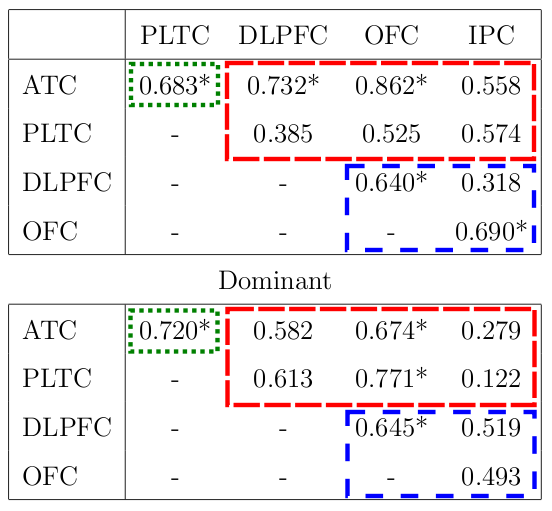
\includegraphics[width=0.75\linewidth]{figures/subnet_table_2.png}
\caption{Group-wise correlations of activation t-values under all conditions. * $p<0.05$. Cortical regions include orbital frontal (OFC), anterior temporal (ATC), posterior lateral temporal (PLTC), dorso-lateral prefrontal (DLFPC), and inferior partietal (IPC). A green dotted line identifies the language subnetwork connections, a spaced blue dashed line identifies the connections of the decision-making subnetwork and a red dashed line identifies connections between the language and decision-making subnetworks }
\label{table:popcorrt}
\end{center}
\end{table}

\begin{figure}[h]
\begin{center}
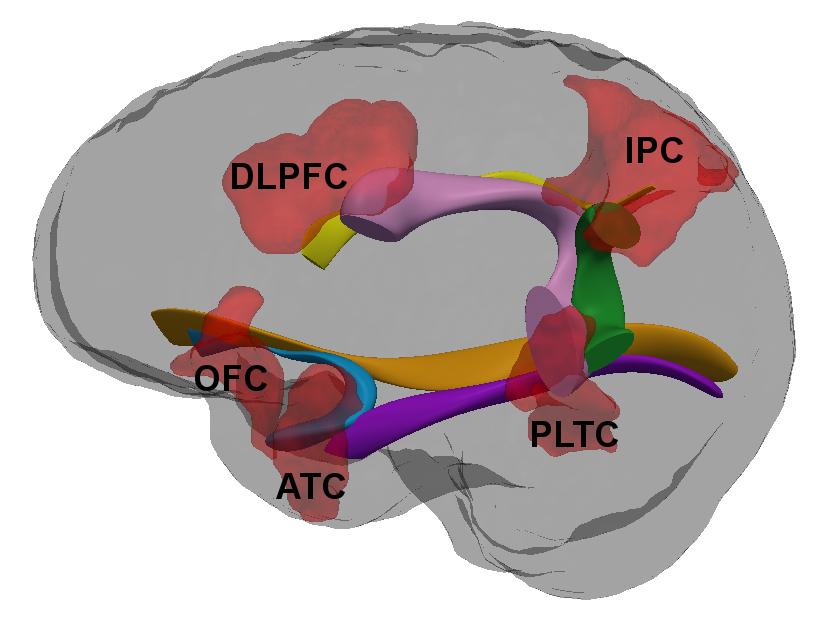
\includegraphics[width=1.0\linewidth]{figures/big_homo_labeled.png}
\caption{Functionally activated cortical regions (shown in red) were used to identify white matter fiber bundles that connected any two activated regions of interest. This resulted in the identification of six white matter projections for which mean fractional anisotropy (FA) was calculated. This network included the uncinate fasciculus (blue, FA=$0.397 \pm 0.092$), arcuate fasciculus (pink, FA=$0.459 \pm 0.151$), inferior frontal-occiptal fasciculus (orange, FA=$0.646 \pm 0.122$), inferior longitudinal fasciculus (purple, FA=$0.479 \pm 0.142$), superior longitudinal fasciculus (yellow, FA=$0.523 \pm 0.068$) and the arcuate fasciculus vertical (green, FA=$0.511 \pm 0.099$).}
\label{fig:networkmodel}
\end{center}
\end{figure}

\begin{figure}[h]
\begin{center}
\begin{tabular}{ c c }
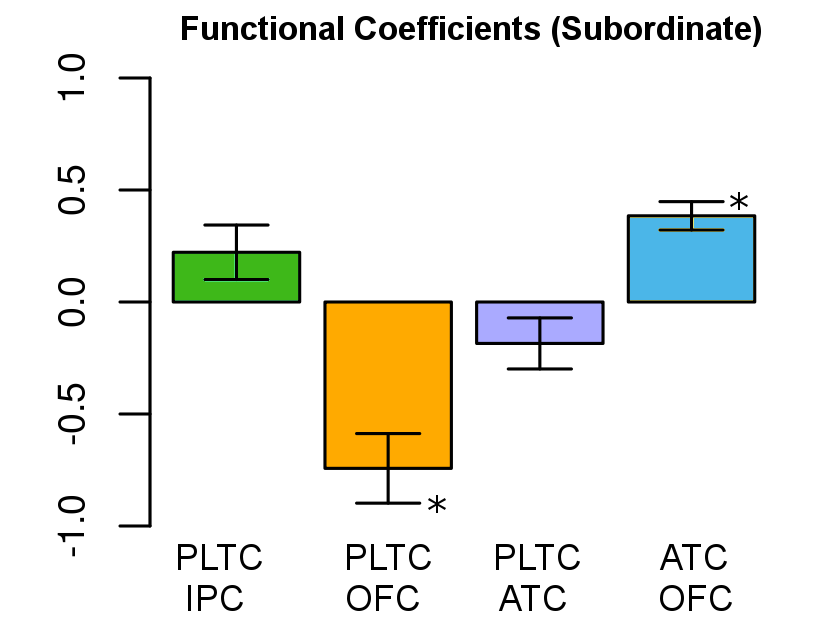
\includegraphics[width=0.45\linewidth]{figures/FC_Subordinate2.png} &
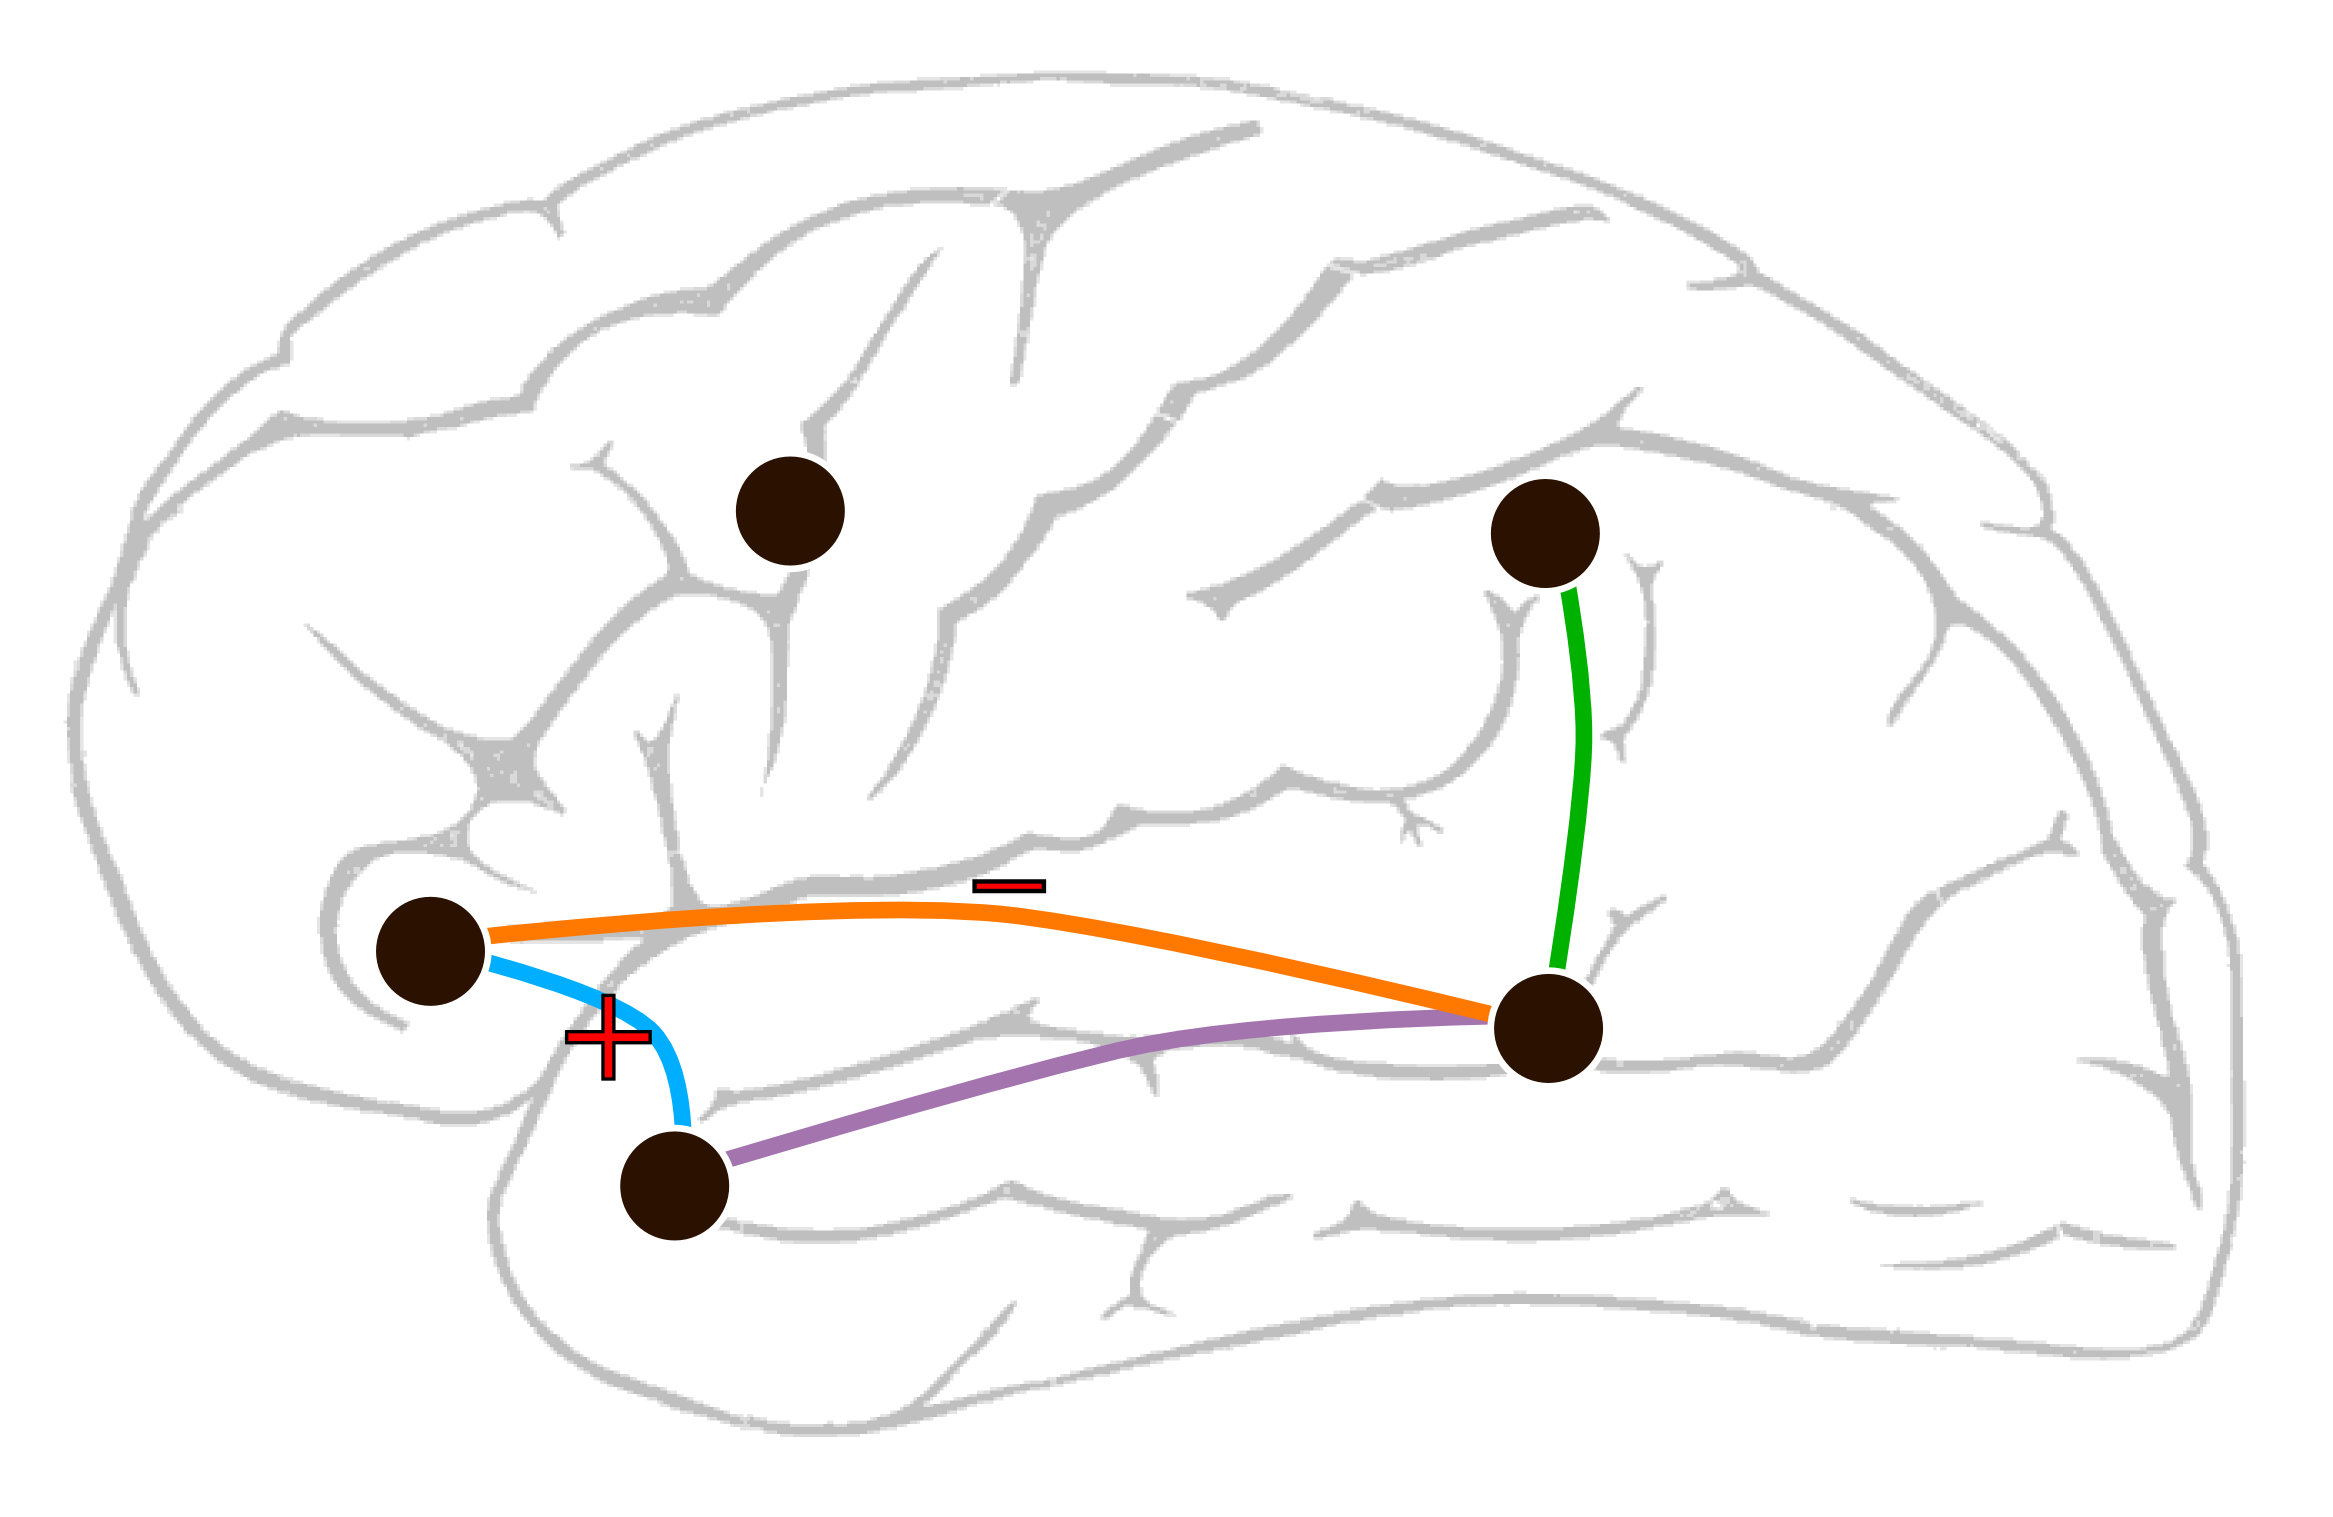
\includegraphics[width=0.45\linewidth]{figures/func_diag2.png} 
\end{tabular}
\caption{Stepwise multiple linear regression analysis examining performance in the subordinate context and functional connectivity between regions connected by a white matter fiber tract resulted in a model including the vertical aspect of the arcuate fasciculus (AFV), IFO, IFL and UNC. * $p<0.05$}
\label{fig:mlr_fc}
\end{center}
\end{figure}

\begin{figure}[h]
\begin{center}
\begin{tabular}{ c c }
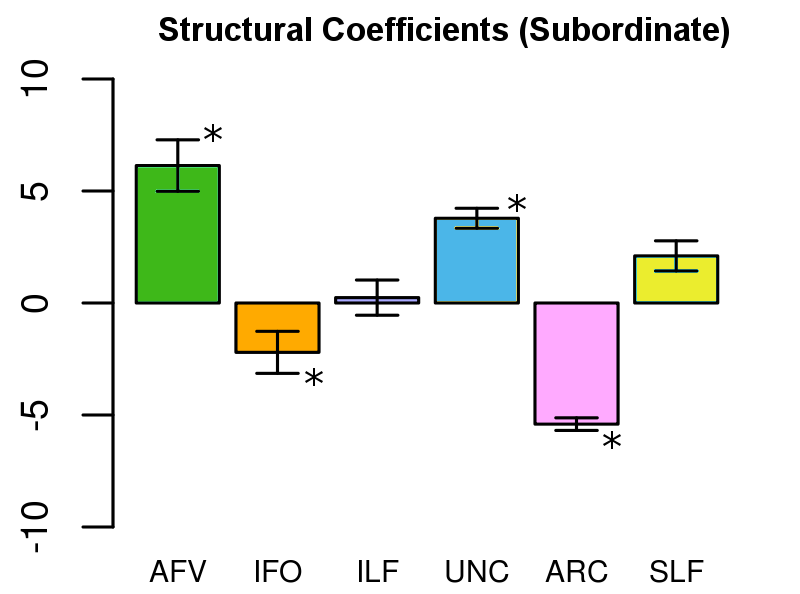
\includegraphics[width=0.45\linewidth]{figures/FA_Subordinate2.png} &
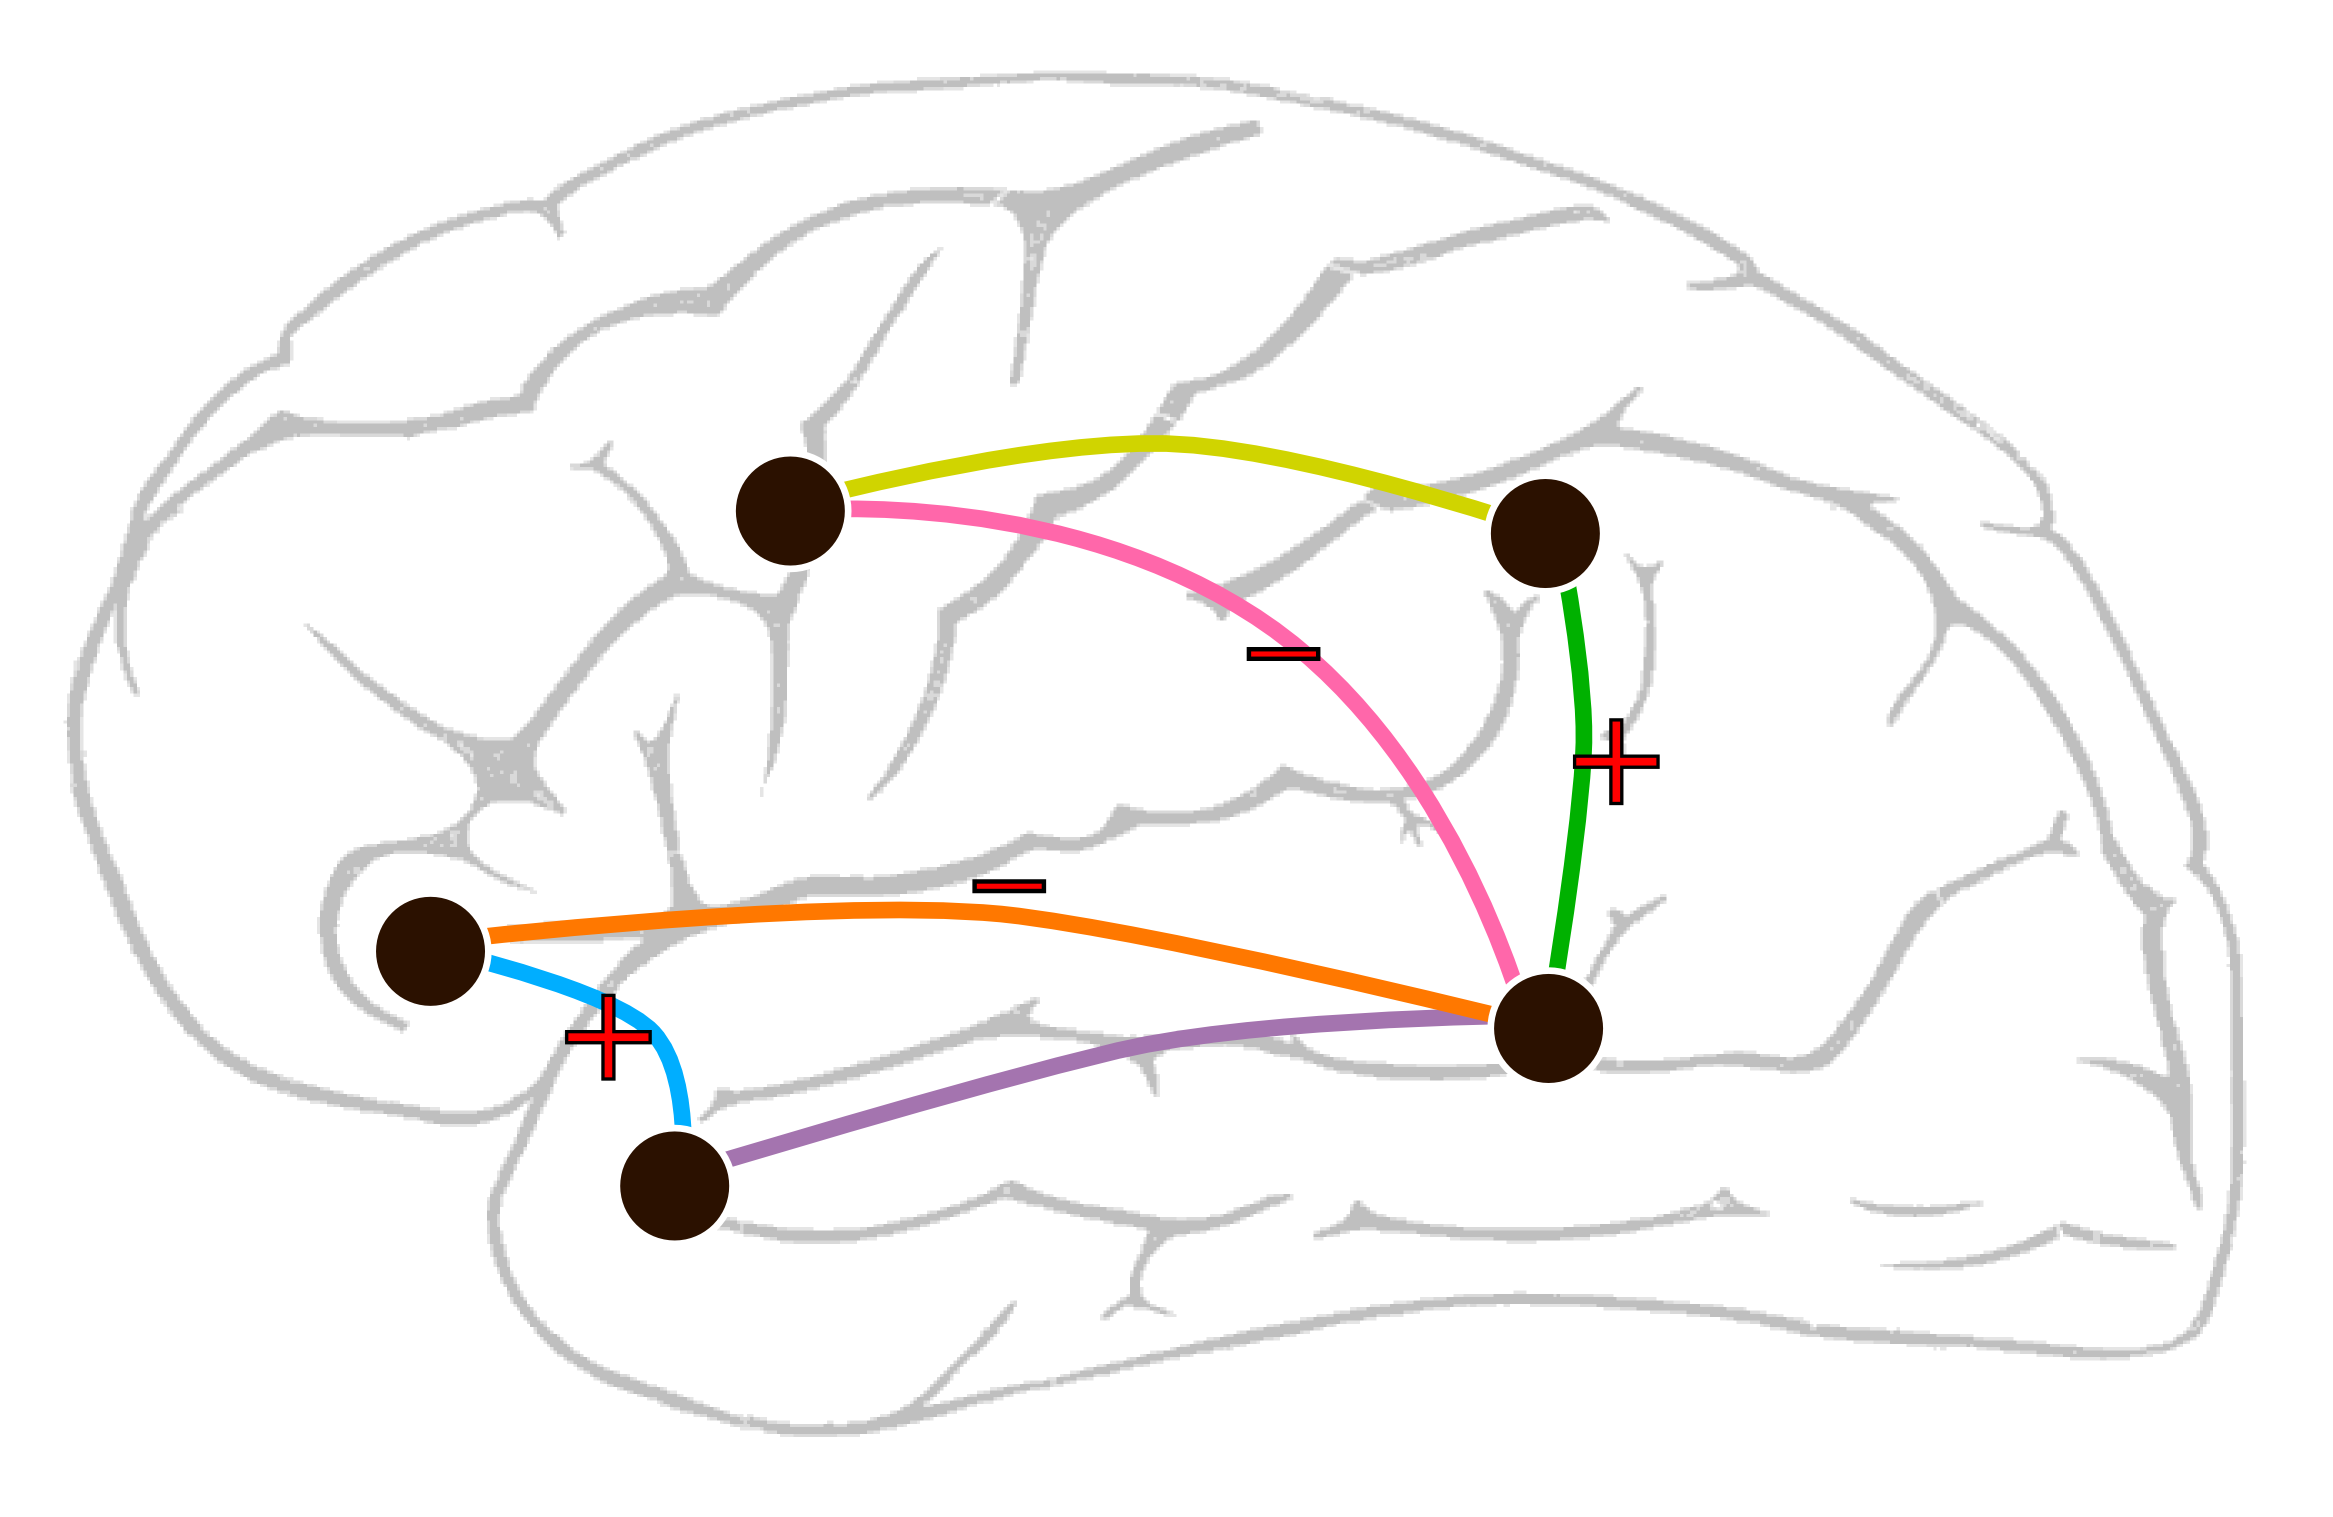
\includegraphics[width=0.45\linewidth]{figures/struct_diag2.png}
\end{tabular}
\caption{Stepwise multiple linear regression analysis examining performance in the subordinate context and tract averaged FA implicated all biological connections in the network: uncinate fasciculus (UNC), arcuate fasciculus (ARC), superior longitudinal fasciculus (SLF), inferior longitudinal fasciculus (ILF), inferior frontal-occipital fasciculus (IFO) and the arcuate fasciculus vertical (AFV). The coefficients for each structure are illustrated here. *Indicates an individually significant fiber tract ($p<0.05$).}
\label{fig:mlr_fa}
\end{center}
\end{figure}



\end{document}

%%
%% End of file `elsarticle-template-2-harv.tex'.
